\documentclass{article}
\usepackage{graphicx} 
\usepackage{amsmath} 
\usepackage{pgfplots} 
\pgfplotsset{compat=1.18} 
\usepackage{titlesec}
\titlespacing*{\section}{0pt}{10pt}{5pt} 
\titlespacing*{\subsection}{0pt}{5pt}{2pt} 

\title{Quiz 2 / MAC 2313 / Spring 2025}
\author{Caitlin Box}
\date{January 22, 2025}
\begin{document}
\maketitle

\section{For 1-5, let $\vec{u}$ be the standard position vector terminating at (5,-7)}

\begin{center}
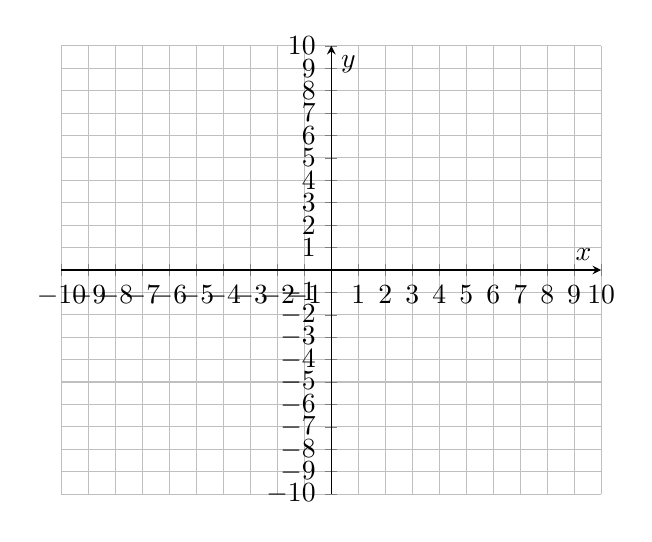
\begin{tikzpicture}
    \begin{axis}[
        axis lines = middle,
        xmin = -10, xmax = 10,
        ymin = -10, ymax = 10,
        grid = both,
        xlabel = {$x$},
        ylabel = {$y$},
        xtick={-10,-9,...,10},
        ytick={-10,-9,...,10},
    ]
    \end{axis}
\end{tikzpicture}
\end{center}

\subsection{Draw $\vec{u}$ on the axis provided. (ONLY $\vec{u}$)}
\subsection{Find the magnitude of $\vec{u}$ (Show appropriate work.)}  
\vspace{1cm}
\subsection{The \textbf{unit vector} in the direction of $\vec{u}$ is \_\_\_ $\hat{i}$ + \_\_\_ $\hat{j}$.}
\vspace{1cm}
\subsection{Suppose $\vec{v}$ initiates at (-1,2) and is \textbf{EQUIVALENT} to $\vec{u}$, then $\vec{v}$ terminates at (\_\_\_, \_\_\_)}
\vspace{1cm}
\subsection{$\vec{u}$ - $\vec{v}$ = \_\_\_ (Give your answer in component form.)}
\newpage


\section{For 6-9, let $\vec{a}$ = $\hat{i}$ + 3$\hat{j}$ - $\hat{k}$ and $\vec{b}$ = 2$\hat{i}$ + $\hat{j}$. Show all appropriate work.}
\vspace{1cm}
\subsection{$\vec{a}$ $\cdot$ $\vec{b}$ = \_\_\_}
\vspace{3cm}
\subsection{Find the angle between $\vec{a}$ and $\vec{b}$.}
\vspace{3cm}
\subsection{Find the scalar projection of $\vec{b}$ onto $\vec{a}$.}
\vspace{3cm}
\subsection{Find the vector projection of $\vec{b}$ onto $\vec{a}$.}

\end{document}
